\documentclass[aps,prd,preprint,superscriptaddress,tightenlines,nofootinbib,floatfix]{revtex4}

%%%%%%%%%%%%%% Use for PRL
%\documentclass[aps,prl,twocolumn,superscriptaddress,showpacs]{revtex4}

%%%%%%%%%%%%%% Use for PRD submission
%\documentclass[aps,prd,preprint,nopreprintnumbers,nofootinbib,showpacs]{revtex4}
%%%%%%%%%%%%%% Use for PRD formatting tables and figures in 2 column
%\documentclass[aps,prd,twocolumn,nofootinbib,showpacs]{revtex4}

\usepackage{graphicx}% Include figure files
\usepackage{dcolumn}% Align table columns on decimal point
\usepackage{bm}% bold math
\usepackage{multirow}% multirow table entries
\usepackage{amsmath}
\usepackage{color}

\begin{document}

%-Definitions-----------------------------------------------------------

\newcommand{\etal}{{\it et al.}}
\newcommand{\ee}{$e^+e^-$}
\newcommand{\mm}{$\mu^+\mu^-$}

\newcommand{\subs}[1]{{\mbox{\scriptsize #1}}}
\newcommand{\re}{\mathrm{Re\:}}
\newcommand{\gee}{$\Gamma_{ee}$}
\newcommand{\ups}{$\Upsilon$}
\newcommand{\uone}{$\Upsilon(1S)$}
\newcommand{\utwo}{$\Upsilon(2S)$}
\newcommand{\uthree}{$\Upsilon(3S)$}
\newcommand{\mpprec}{$m_\subs{$\pi\pi$-rec}$}
\newcommand{\bbar}{$b\bar{b}$}
\newcommand{\inv}{$^{-1}$}
\newcommand{\twotoone}{$\Upsilon(2S) \to \pi^+\pi^- \Upsilon(1S)$}
\newcommand{\pip}{$\pi^+\pi^-$}
\newcommand{\tautau}{$\tau^+\tau^-$}
\newcommand{\dxy}{$d_{XY}$}
\newcommand{\dz}{$d_Z$}

%-----------------------------------------------------------------------
%-----------------------------------------------------------------------
%-----------------------------------------------------------------------

%\preprint line(s) will be ignored for PRL/PRD
%\preprint{CLEO Draft YY-NNA} % For paper draft CBX YY-NN -> Draft YY-NNA
%\preprint{CLEO CONF YY-NN}   % For conference papers
%\preprint{ICHEP ABSnnn}      % For conference papers
%% \preprint{CLNS 05/XXXX; CLEO 05-XX}       % for CLNS notes
%% \preprint{EPS-XXX}         % for CLNS notes
\preprint{CBN 05-15}

\title{What the Upsilon Scans Teach Us About CESR at 5 GeV}

%% \thanks{Archived as hep-ex/XXXXXXX; 
%% submitted to {\it Phys. Rev. Q}}

%-------- INSERT HERE ------------
% Your author list goes here  REMOVE EVERYTHING to END INSERT and
% replace with your authorlist (ask cleoac).

\author{J.~Pivarski}
\affiliation{F.~R.~Newman Laboratory for Elementary-Particle Physics, Ithaca, New York 14850-8001}
%\author{(CLEO Collaboration)} %FOR PRD_SPECIAL_CHANGEME
\collaboration{CLEO Collaboration} %FOR PRL,CLNS
\noaffiliation

%\author{John Doe}
%\affiliation{Physics Department, Cornell University
%Ithaca, New York 14853}
%\author{(CLEO Collaboration)}     %FOR PRD_SPECIAL_CHANGEME
%\collaboration{CLEO Collaboration} %FOR PRL and CLNS (superscriptaddress)
%\noaffiliation

%-------- END INSERT ------------

%please hard code the date when you have a final draft and submit to CLEOAC
\date{\today}

%---------------------------------------------------------------------
%
%\abstract
%
%---------------------------------------------------------------------

\begin{abstract} 
We present fit results of \uone, \utwo, and \uthree\ lineshape scans
that are relevant for studies of CESR.  The beam energy spread
($\sigma_E/E$) is 20\% narrower than expected, though its relationship
with beam energy is linear, with a slope of (119 $\pm$ 75) $\times$
10$^{-6}$ GeV\inv.  We also find that the beam energy measurement
varies by $\sim$0.3 MeV/5 GeV from week to week, but less than 0.07
MeV within a 10-hour scan period (68\% C.L.).  Measured \ups\ masses/2
are lower than PDG masses/2 by (0.20 $\pm$ 0.14) MeV, (-0.46 $\pm$
0.20) MeV, and (-1.51 $\pm$ 0.33) MeV for the \uone, \utwo, and
\uthree\ respectively.
\end{abstract}
\pacs{13.20.He}  %% what's this?
\maketitle

\section{Introduction}

\begin{figure}[t]
  \begin{center}
    \includegraphics[width=0.9\linewidth]{three_resonances}
  \end{center}
  \caption{\label{upsilons} Fits to the \uone, \utwo, and \uthree\
    (left to right) including the initial state radiation tail.  The
    three plot windows are equally wide.  The ``hadronic
    cross-section'' background contains some radiative bhabhas.}
\end{figure}

From November 2001 to August 2002, CESR performed detailed scans of the
three narrow \ups\ resonances to precisely measure their di-electron
widths, \gee.  Because these resonances are very narrow (25--50 keV),
they can also be used as delta-function probes of the CESR beams.  We
used their fitted widths to measure the beam energy spread directly,
and their fitted masses to correct the beam energy measurement, since
the \ups\ masses are very well known.

For the \gee\ analysis, we fit the three resonances to a convolution
of a Breit-Wigner peak, an initial state radiation (ISR) tail, and a
Gaussian beam energy spread (see Figure \ref{upsilons}) \cite{kb}.
This three-way convolution accounts for a widening of the peak due to
the ISR tail (and, to a tiny extent, the Breit-Wigner width) and a
shift in the peak maximum toward higher energies, due to the ISR tail.
In this document, we will quote beam energy spreads as single-beam
spreads $\sigma_E$ with the ISR tail (and Breit-Wigner width) removed,
and \ups\ masses in terms of single-beam energies with the ISR tail
removed.  Since we perform all fits in the center-of-mass, this means
that we divide our fitted widths by $\sqrt{2}$ and our fitted masses
by $2$.  (With the exception of Figure \ref{upsilons}, we only quote
single-beam quantities in this document.)

The data were acquired in small, independent, weekly scans (defined in
terms of run numbers and dates in Appendix \ref{sec:scans}).  In
principle, one could fit each week separately, but this would not be
an optimal use of the data, particularly the continuum ($\sim$10 MeV
below resonance) and high-energy tail (25--50 MeV above resonance)
points, which are not sensitive to small shifts in beam energy.
Instead, we fit all scans of a given resonance in a single fit, with
separate \ups\ mass parameters for each weekly scan, i.e., the
``calibration'' of each week's beam energy measurement is allowed to
float.  The following is an exhaustive list of floating fit
parameters: lineshape area (\gee), background level, beam energy
spread ($\sigma_E$), and a parameter representing $M_\Upsilon$(PDG)
$-$ $M_\Upsilon$(measured) for each weekly scan (12 for \uone, 6 for
\utwo, and 7 for \uthree).

Cross-section measurements are described in \cite{me}.  The most
pertinent result from that analysis is the conclusion that
cross-section measurements are very reproducible: the largest
cross-section jitter the data can support is $\pm$0.03 nb (68\% C.L.\
upper bound), whereas the statistical error in most cross-section
measurements is 0.2 nb.  Therefore, we will treat all cross-section
measurements as being limited only by statistical errors.

In this note, we will present measurements of beam energy spreads
(Section \ref{sec:spread}), reproducibility of the beam energy
measurement from one week to the next (Section \ref{sec:weekly}), and
within a 10-hour scan (Section \ref{sec:tenhour}).  We hope this will
provide useful information about the CESR beams at 5 GeV.

\section{Measurements of Beam Energy Spread} \label{sec:spread}

Single-beam energy spreads, expressed as a fraction of beam energy
($\sigma_E/E$), were measured to be (565 $\pm$ 4) $\times$ 10$^{-6}$,
(587 $\pm$ 12) $\times$ 10$^{-6}$, and (616 $\pm$ 14) $\times$
10$^{-6}$ for the \uone, \utwo, and \uthree, respectively (beam
energies are 4.7302, 5.0116, and 5.1776 GeV).  These are plotted in
Figure \ref{beamenergyspread}, along with the CESRV prediction,
extrapolated from the {\tt CESRC\_3S\_V2 lattice}.  Although the
predicted beam energy spread is 20\% too high, the three measurements
are consistent with proportional scaling ($\sigma_E/E \propto E$),
with a slope of (119 $\pm$ 75) $\times$ 10$^{-6}$ GeV\inv.

\begin{figure}[p]
  \begin{center}
    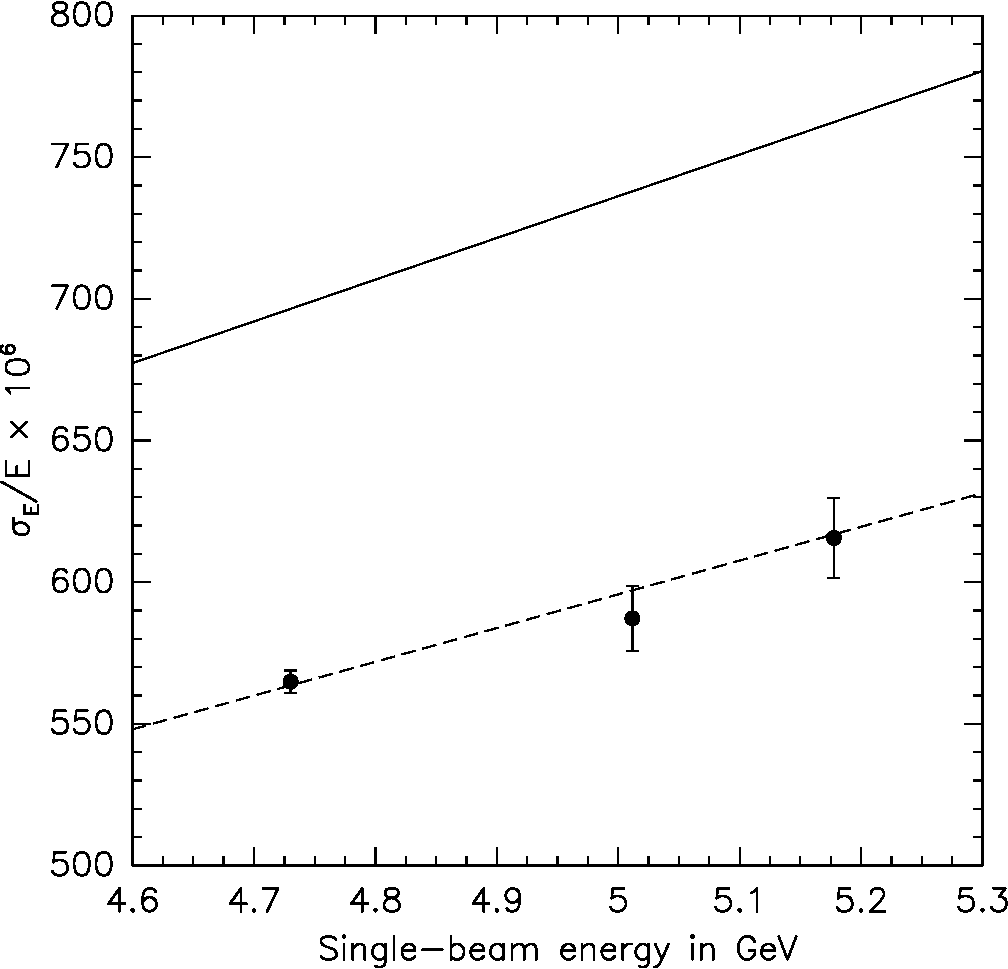
\includegraphics[width=\linewidth]{beamenergyspread}
  \end{center}
  \caption{\label{beamenergyspread} Beam energy spread versus beam
  energy, compared to the CESRV prediction (solid line, extrapolated
  from $\Upsilon(3S)$) and a fit (dotted line).}
\end{figure}

\begin{figure}[p]
  \includegraphics[width=\linewidth]{../plots/deltaei_cesr}
  \caption{\label{widths} Beam energy spread ($\sigma_E/E$) of each
  weekly scan (points), compared to the output of a combined fit for
  $\sigma_E/E$ (dotted lines).  The {\tt apr03} scan is missing
  measurements on the high-energy side of the peak (see Figure
  \ref{postage}).}
\end{figure}

\begin{table}[p]
  \begin{center}
    \renewcommand{\arraystretch}{1.25}
    \begin{tabular}{c | c c}
\mbox{\hspace{0.5 cm}} Scan \mbox{\hspace{0.5 cm}} & \mbox{\hspace{0.5 cm}} Single beam energy spread in MeV \mbox{\hspace{0.5 cm}} & \mbox{\hspace{0.5 cm}} $\sigma_E/E$ $\times$ 10$^{6}$ \mbox{\hspace{0.5 cm}} \\\hline
jan16 & 2.50 $\pm$ 0.08 & 527 $\pm$ 17 \\
jan30 & 2.71 $\pm$ 0.03 & 572 $\pm$ \textcolor{white}{0}5 \\
feb06 & 2.68 $\pm$ 0.04 & 566 $\pm$ \textcolor{white}{0}7 \\
feb13 & 2.59 $\pm$ 0.08 & 547 $\pm$ 15 \\
feb20 & 2.63 $\pm$ 0.04 & 556 $\pm$ \textcolor{white}{0}8 \\
feb27 & 2.70 $\pm$ 0.04 & 569 $\pm$ \textcolor{white}{0}7 \\
mar06 & 2.65 $\pm$ 0.04 & 559 $\pm$ \textcolor{white}{0}8 \\
mar13 & 2.70 $\pm$ 0.03 & 570 $\pm$ \textcolor{white}{0}7 \\
apr03 & 3.07 $\pm$ 0.15 & 649 $\pm$ 31 \\
apr08 & 2.66 $\pm$ 0.09 & 562 $\pm$ 19 \\
apr09 & 2.78 $\pm$ 0.11 & 588 $\pm$ 22 \\
apr10 & 2.62 $\pm$ 0.03 & 553 $\pm$ \textcolor{white}{0}7 \\\hline
may29 & 3.03 $\pm$ 0.11 & 604 $\pm$ 20 \\
jun11 & 2.84 $\pm$ 0.20 & 566 $\pm$ 39 \\
jun12 & 3.01 $\pm$ 0.08 & 600 $\pm$ 16 \\
jul10 & 2.77 $\pm$ 0.12 & 553 $\pm$ 23 \\
jul24 & 2.67 $\pm$ 0.32 & 531 $\pm$ 64 \\
aug07 & 3.00 $\pm$ 0.13 & 597 $\pm$ 26 \\\hline
nov28 & 3.34 $\pm$ 0.11 & 645 $\pm$ 20 \\
dec05 & 3.16 $\pm$ 0.10 & 609 $\pm$ 19 \\
dec12 & 3.20 $\pm$ 0.09 & 618 $\pm$ 18 \\
dec19 & 3.32 $\pm$ 0.13 & 641 $\pm$ 24 \\
dec26 & 2.91 $\pm$ 0.14 & 562 $\pm$ 27 \\
jan02 & 3.24 $\pm$ 0.11 & 625 $\pm$ 21 \\
jan09 & 3.26 $\pm$ 0.09 & 629 $\pm$ 17 \\\hline
    \end{tabular}
  \end{center}
  \caption{\label{widthstab} The data plotted in Figure \ref{widths}.
  The three blocks are \uone, \utwo, and \uthree, top to bottom.}
\end{table}

To see if the beam energy spread changes between scans, we replaced the
single parameter $\sigma_E$ with a separate beam energy spread for
each weekly scan.  The results of this fit are plotted in Figure
\ref{widths} and listed in Table \ref{widthstab}.  All beam energy
spreads seem to be consistent with a single $\sigma_E$ except for
{\tt apr03}.

The {\tt apr03} scan only includes measurements on the low-energy side
of the peak (see Figure \ref{postage} in Appendix \ref{sec:scans}).
This is not because any runs were lost, but the high-side points
differ from their design energy by a factor of two (e.g.\ 13 MeV above
the resonance mass instead of 6 MeV).  (This may have been due to a
miscommunication about single-beam energies and center-of-mass
energies.)  The beam energy spread in this scan can not be adequately
measured, though it is surprising that the fitted uncertainty does not
compensate for this effect.  (These are MINOS errors; they are allowed
to be asymmetric and non-linear.)

Removing this outlier (2.6$\sigma$), the reduced $\chi^2$ of \uone\
beam energy spreads is 13.9/10 = 1.4.  The reduced $\chi^2$ of \utwo\
and \uthree\ beam energy spreads is 4.6/5 = 0.92 and 8.7/6 = 1.5,
respectively.  The reduced $\chi^2$ for all three is 27.2/21 = 1.3,
which is consistent with a single beam energy spread (with a 16\%
C.L.).

\section{Beam Energy Measurement Reproducibility}

\subsection {From Week to Week} \label{sec:weekly}

As previously mentioned, our fits for \gee\ allow $M_\Upsilon$ from
each week to float, so the reproducibility of the beam energy
measurement can be read directly from the fit values.  These are
plotted in Figure \ref{centroids} and listed in Table
\ref{centroidstab} as differences from the PDG \ups\ mass.

\begin{figure}[p]
  \includegraphics[width=\linewidth]{../plots/deltam_cesr}
  \caption{\label{centroids} Weekly scan measurements of $M_\Upsilon$
    as a difference from the PDG $M_\Upsilon$, divided by 2 for
    single-beam energy measurement shifts in MeV.  These are
    corrections that need to be {\it added} to beam energy
    measurements.}
\end{figure}

\begin{table}[p]
  \begin{center}
    \renewcommand{\arraystretch}{1.25}
    \begin{tabular}{c | c}
\mbox{\hspace{0.5 cm}} Scan \mbox{\hspace{0.5 cm}} & \mbox{\hspace{0.5 cm}} ($M_\Upsilon$(PDG) $-$ $M_\Upsilon$(measured))/2 in MeV \mbox{\hspace{0.5 cm}} \\\hline
jan16 & 0.12 $\pm$ 0.06 \\
jan30 & 0.27 $\pm$ 0.05 \\
feb06 & 0.12 $\pm$ 0.05 \\
feb13 & 0.03 $\pm$ 0.05 \\
feb20 & 0.08 $\pm$ 0.05 \\
feb27 & 0.06 $\pm$ 0.05 \\
mar06 & 0.11 $\pm$ 0.06 \\
mar13 & 0.28 $\pm$ 0.05 \\
apr03 & 0.45 $\pm$ 0.07 \\
apr08 & 0.39 $\pm$ 0.06 \\
apr09 & 0.22 $\pm$ 0.06 \\
apr10 & 0.37 $\pm$ 0.05 \\\hline
may29 & -0.52 $\pm$ 0.10 \\
jun11 & -0.54 $\pm$ 0.08 \\
jun12 & -0.76 $\pm$ 0.09 \\
jul10 & -0.38 $\pm$ 0.06 \\
jul24 & -0.34 $\pm$ 0.11 \\
aug07 & -0.19 $\pm$ 0.10 \\\hline
nov28 & -1.15 $\pm$ 0.27 \\
dec05 & -2.03 $\pm$ 0.12 \\
dec12 & -1.59 $\pm$ 0.16 \\
dec19 & -1.05 $\pm$ 0.17 \\
dec26 & -1.47 $\pm$ 0.11 \\
jan02 & -1.35 $\pm$ 0.15 \\
jan09 & -1.24 $\pm$ 0.20 \\\hline
    \end{tabular}
  \end{center}
  \caption{\label{centroidstab} The data plotted in Figure
  \ref{centroids}.  The three blocks are \uone, \utwo, and \uthree,
  top to bottom.}
\end{table}

These measurements are not consistent with a single mass, so we can
infer that the calibration of the single-beam energy measurement does
shift by about 0.3 MeV from one week to the next.  (The RMS shift is
0.3 MeV; the beam energy measurement sometimes appears to drift
smoothly over long timescales.)

The average $M_\Upsilon$(PDG) $-$ $M_\Upsilon$(measured) is not zero,
so we can also infer a correction to the beam energy measurement.
Beam energy measurements in the \uone\ region need to be increased by
(0.20 $\pm$ 0.02 $\pm$ 0.14) MeV, measurements in the \utwo\ region
need to be decreased by (0.46 $\pm$ 0.04 $\pm$ 0.20) MeV, and
measurements in the \uthree\ region need to be decreased by (1.51
$\pm$ 0.06 $\pm$ 0.33) MeV, where the first uncertainty is statistical
and the second is the RMS of week-by-week variations.  These
corrections are plotted in Figure \ref{correction} and are
\begin{equation}
  \mbox{correct beam energy}(E_\subs{beam}) = E_\subs{beam} + (15 \pm
  3) \mbox{ MeV} + (-0.0031 \mp 0.0007) \times E_\subs{beam}
  \label{eqncorrect}
\end{equation}
if fitted to a line, where $E_\subs{beam}$ is the output of the beam
energy program.  The uncertainties in the intercept and slope are
almost exactly anticorrelated.  (We are not recommending the
application of this extrapolation far from the \ups\ region!)

\begin{figure}[p]
  \begin{center}
    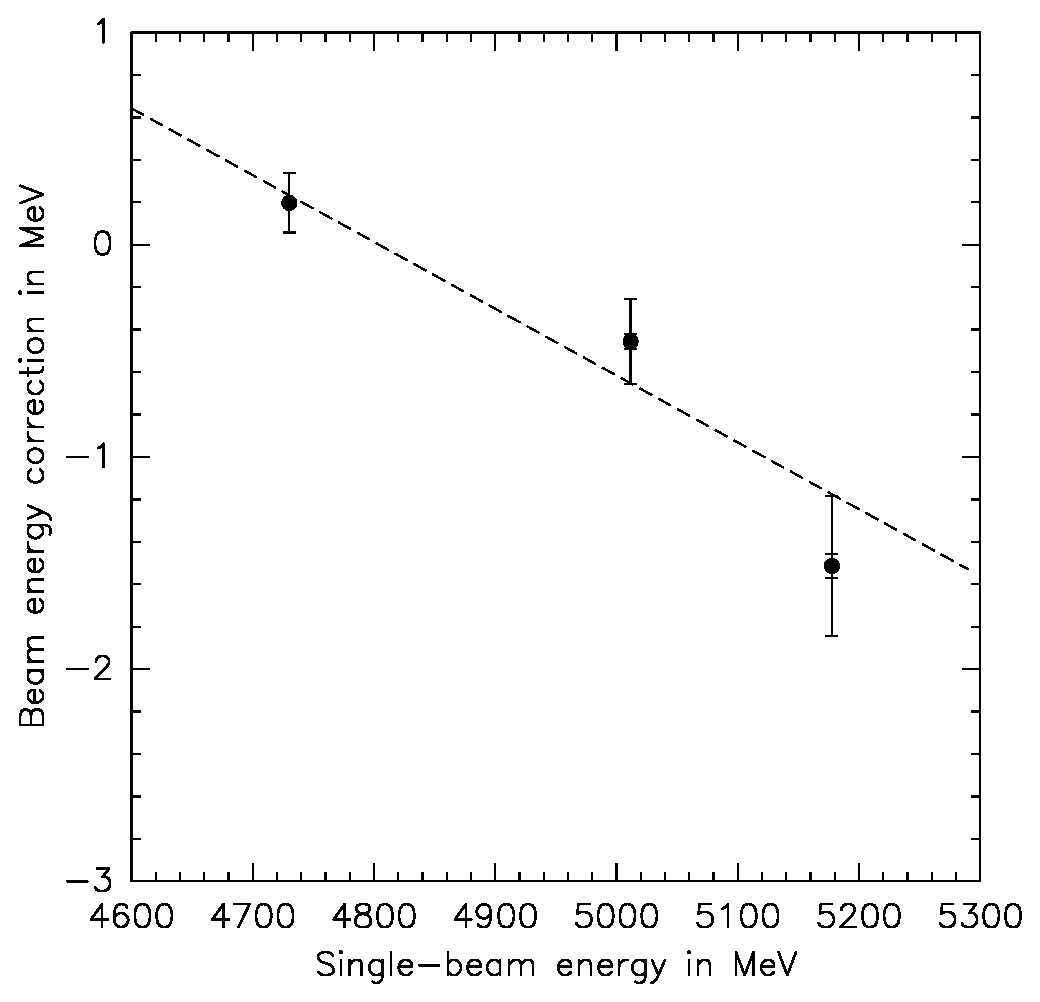
\includegraphics[width=\linewidth]{energycorrection}
  \end{center}
  \caption{\label{correction} A fit to the beam energy correction.
    Inner error bars are purely statistical, outer error bars
    represent the RMS spread in measurement from week to week.  This
    correction should be {\it added} to the single-beam energy
    measurement (see Equation \ref{eqncorrect}).}
\end{figure}

\subsection{Within a 10-Hour Scan} \label{sec:tenhour}

The \gee\ analysis would be sensitive to mismeasurements of beam
energy during a scan, so we chose a scan technique that would allow us
to check the beam energy measurement with the scan data itself.  Most
weekly scans included a repeated energy point (sometimes more than
one), on the shoulder of the \ups\ lineshape where the derivative is
at a maximum, usually at the beginning and end of the scan.  If the
calibration of the beam energy measurement shifts during a scan, the
second cross-section measurement will differ from the first.  We
calculate an ``energy calibration shift'' from a pair of measurements
by
\begin{equation}
  \mbox{calibration shift} = \frac{\sigma_2 - \sigma_1}{f'(E_\subs{beam})} - (E_\subs{beam 2} - E_\subs{beam 1})
  \label{miscaleqn}
\end{equation}
where $f'(E_\subs{beam})$ is the derivative of the lineshape at the
pair's (average) beam energy, $\sigma_1$ and $\sigma_2$ are
cross-section measurements, and $E_\subs{beam 1}$ and $E_\subs{beam
2}$ are the measured beam energies (2 is always later in time than 1).
Since the cross-section measurements are statistics-limited, the
calibration shift measurements will be as well.

The scan data contain 30 pairs of repeated measurements, which we
translate into 30 beam energy calibration shifts using Equation
\ref{miscaleqn} (plotted in Figure \ref{miscalhours} and listed in
Table \ref{miscaltab}).  They are all consistent with zero shift, as
their pulls (shift divided by uncertainty in shift) form a unit
Gaussian (see Figure \ref{miscalpull}).  There is also no apparent
dependence on the time between measurements.

\begin{figure}[p]
  \begin{center}
    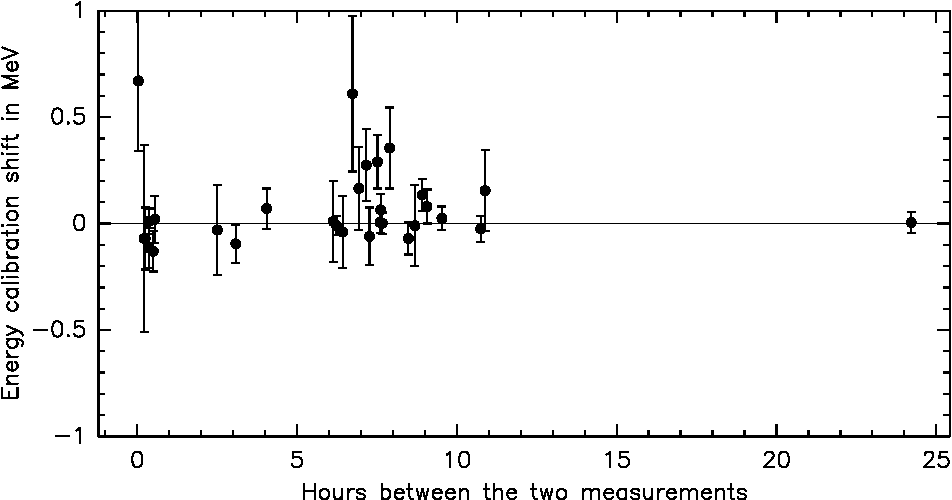
\includegraphics[width=0.9\linewidth]{miscal}
  \end{center}
  \caption{\label{miscalhours} Beam energy calibration shifts, as
    determined from thirty pairs of repeated cross-section
    measurements (plotted versus time).}
\end{figure}

\begin{figure}[p]
  \begin{center}
    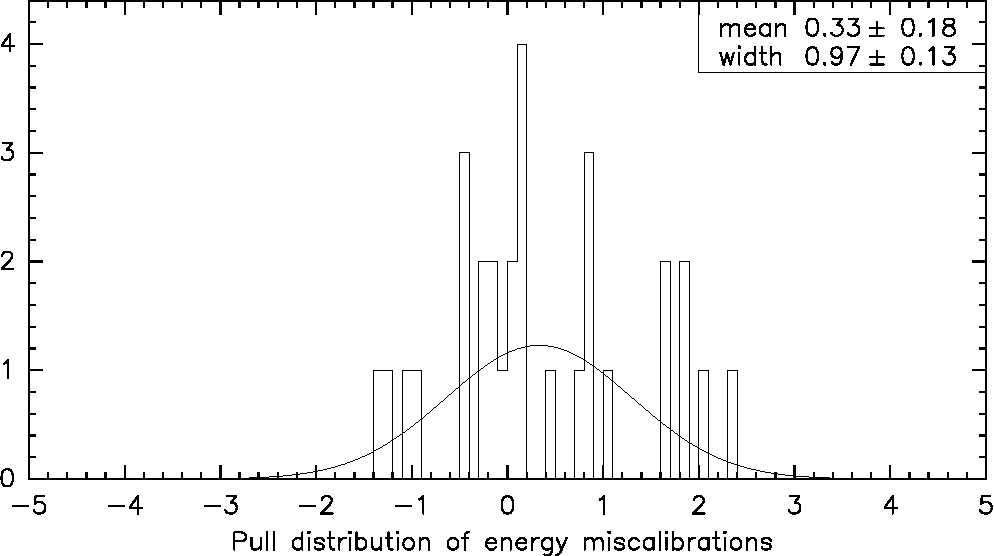
\includegraphics[width=0.9\linewidth]{miscalpull}
  \end{center}
  \caption{\label{miscalpull} Pull distribution of beam energy
    calibration shifts.}
\end{figure}

\begin{table}[p]
  \begin{center}
    \renewcommand{\arraystretch}{1.25}
    \begin{tabular}{c c c}
\mbox{\hspace{0.5 cm}} Minutes between measurements \mbox{\hspace{0.5 cm}} & Energy calibration shift \mbox{\hspace{0.5 cm}} & \mbox{\hspace{0.5 cm}} Weekly scan \mbox{\hspace{0.5 cm}} \\\hline
   2 &  0.67  $\pm$ 0.33  & jan02 \\
  13 & -0.07  $\pm$ 0.44  & jan09 \\
  15 & -0.07  $\pm$ 0.145 & aug07 \\
  22 &  0.01  $\pm$ 0.06  & apr03 \\
  22 & -0.115 $\pm$ 0.095 & may29 \\
  30 & -0.13  $\pm$ 0.095 & jul24 \\
  33 &  0.02  $\pm$ 0.11  & jan16 \\
 150 & -0.03  $\pm$ 0.21  & dec05 \\
 185 & -0.095 $\pm$ 0.09  & jan30 \\
 243 &  0.07  $\pm$ 0.095 & feb06 \\
 368 &  0.01  $\pm$ 0.19  & dec26 \\
 374 & -0.01  $\pm$ 0.045 & feb20 \\
 386 & -0.04  $\pm$ 0.17  & dec26 \\
 404 &  0.61  $\pm$ 0.365 & dec26 \\
 416 &  0.165 $\pm$ 0.195 & dec26 \\
 430 &  0.275 $\pm$ 0.17  & jan02 \\
 436 & -0.06  $\pm$ 0.135 & apr08 \\
 451 &  0.29  $\pm$ 0.125 & apr09 \\
 456 &  0.005 $\pm$ 0.05  & feb06 \\
 457 &  0.065 $\pm$ 0.075 & mar06 \\
 460 &  0.002 $\pm$ 0.05  & feb13 \\
 474 &  0.355 $\pm$ 0.19  & dec19 \\
 509 & -0.07  $\pm$ 0.075 & feb27 \\
 521 & -0.01  $\pm$ 0.19  & jan09 \\
 535 &  0.135 $\pm$ 0.075 & jan16 \\
 544 &  0.08  $\pm$ 0.08  & mar13 \\
 572 &  0.025 $\pm$ 0.055 & jan30 \\
 645 & -0.025 $\pm$ 0.06  & jul10 \\
 653 &  0.155 $\pm$ 0.19  & dec12 \\
1453 &  0.005 $\pm$ 0.05  & jun11, jun12 \\\hline
    \end{tabular}
  \end{center}
  \caption{\label{miscaltab} The data plotted in Figure
  \ref{miscalhours}.}
\end{table}

We applied two methods to set an upper limit on beam energy
measurement jitter.  First, we defined a negative log likelihood for
the 30 measurements by
\begin{equation}
  \mbox{-log likelihood}(\delta_E) = \sum_{i=1}^{30} -\ln \left(\frac{1}
  {\sqrt{2\pi ({\delta_{s_i}}^2 + {\delta_E}^2)}} \exp\left(
  -s_i^2 / 2 / ({\delta_{s_i}}^2 + {\delta_E}^2) \right) \right)
\end{equation}
where $s_i$ $\pm$ $\delta_{s_i}$ are the calibration shift
measurements listed in Table \ref{miscaltab}, and $\delta_E$ is a
hypothetical random jitter in the measurement.  To raise $L(\delta_E)$
above $L(0)$ by 0.5, a $\delta_E$ of 0.05 MeV is needed.

Another way to calculate the same thing is to define an $S$ factor in
analogy to the PDG's,
\begin{equation}
  S(\delta_E) = \sum_{i=1}^{30} \frac{s_i}{{\delta_{s_i}}^2 +
  {\delta_E}^2} \, \frac{1}{30 - 1} \mbox{.}
\end{equation}
The value of $\delta_E$ needed for $S(\delta_E)$ = 1 is 0.07 MeV.
Because these two methods agree relatively well, we claim that the
68\% C.L.\ upper limit on beam energy measurement shifts (in a 10-hour
period) is 0.07 MeV.

\section{Summary}

We learned from these studies that
\begin{enumerate}
  \item the CESRV beam energy spread prediction is 20\% too wide,

  \item the calibration of the beam energy measurement drifted on the
    order of 0.3 MeV from week to week,

  \item if one desires $\lesssim$ 0.03\% errors in $\Upsilon$ beam
    energy measurements, one must apply the correction in Equation
    \ref{eqncorrect}, and

  \item the calibration of the beam energy measurement drifted less
    than about 0.07 MeV during a 10-hour scan.
\end{enumerate}

\begin{thebibliography}{99}

%% \bibitem{Artamonov:2000cz}
%%   A.~S.~Artamonov {\it et al.}  [OLYA Collaboration],
%%   %``High Precision Mass Measurements in \Psi and\Upsilon Families Revisited,''
%%   Phys.\ Lett.\ B {\bf 474}, 427 (2000)
%%   [arXiv:hep-ex/0001040].
%%   %%CITATION = HEP-EX 0001040;%%

\bibitem{kb} K.~Berkelman, {\it Primer on Onium Widths,} CBX 02-10, and {\it Onium Line Shape Fitting,} CBX 03-12.

\bibitem{me} J.~Pivarski, R.~Patterson, and K.~Berkelman, {\it Di-electron Widths of the Upsilon(1S,2S,3S) Resonances,} CBX 05-41.

\end{thebibliography}

\appendix

\section{Definition of Weekly Scans} \label{sec:scans}

The 25 weekly scan periods referred to throughout this document are
defined in Table \ref{scandates} and presented graphically in Figures
\ref{scanperiods1}--\ref{scanperiods5}.  Mini-plots of each scan are
available in Figure \ref{postage}, just to show what energy points are
available to each.

We defined these periods conservatively by dividing any scan with a
gap of more than 6 hours (during which the beam energy measurement
might shift) into two scans.  In both cases (apr08, apr09, apr10, and
jun11, jun12), we see no significant shift.  Also, all scans,
including on-resonance data, are limited to a total of 48 hours.
(Data beyond 48 hours would only be at the top of the resonance peak,
where the extra statistical precision has diminishing returns for
\gee.)

\begin{table}[t]
  \begin{center}
    \renewcommand{\arraystretch}{1.25}
    \begin{tabular}{c | c | c c}
\mbox{\hspace{0.5 cm}} Scan \mbox{\hspace{0.5 cm}}  & \mbox{\hspace{0.5 cm}} CLEO run range (inclusive) \mbox{\hspace{0.5 cm}}  & \mbox{\hspace{0.25 cm}} StartRun Date \mbox{\hspace{0.1 cm}} & \mbox{\hspace{0.1 cm}} EndRun Date \mbox{\hspace{0.25 cm}} \\\hline % & Biggest gap in hours \\\hline
jan16 & 123164 -- 123178 & 15 Jan 21:21 & 16 Jan 10:07 \\ % & 2.8 \\
jan30 & 123596 -- 123645 & 30 Jan 18:44 & 01 Feb 19:01 \\ % & 1.8 \\
feb06 & 123781 -- 123836 & 06 Feb 21:24 & 08 Feb 21:41 \\ % & 1.6 \\
feb13 & 124080 -- 124092 & 19 Feb 22:23 & 20 Feb 08:29 \\ % & 0.3 \\
feb20 & 124102 -- 124159 & 20 Feb 22:09 & 22 Feb 22:29 \\ % & 1.9 \\
feb27 & 124279 -- 124338 & 27 Feb 22:08 & 01 Mar 22:03 \\ % & 1.1 \\
mar06 & 124436 -- 124495 & 06 Mar 22:48 & 08 Mar 22:20 \\ % & 2.8 \\
mar13 & 124625 -- 124681 & 13 Mar 22:34 & 15 Mar 22:37 \\ % & 1.3 \\
apr03 & 125119 -- 125127 & 02 Apr 21:58 & 03 Apr 06:11 \\ % & 0.7 \\
apr08 & 125254 -- 125262 & 08 Apr 21:44 & 09 Apr 06:41 \\ % & 0.4 \\
apr09 & 125285 -- 125295 & 09 Apr 23:02 & 10 Apr 07:58 \\ % & 0.4 \\
apr10 & 125303 -- 125358 & 10 Apr 20:39 & 12 Apr 20:44 \\\hline % & 1.6 \\\hline
may29 & 126449 -- 126508 & 29 May 18:20 & 31 May 18:28 \\ % & 2.4 \\
jun11 & 126776 -- 126783 & 11 Jun 20:04 & 12 Jun 05:51 \\ % & 0.4 \\
jun12 & 126814 -- 126871 & 12 Jun 18:57 & 14 Jun 19:16 \\ % & 1.7 \\
jul10 & 127588 -- 127615 & 10 Jul 19:42 & 11 Jul 18:28 \\ % & 1.2 \\
jul24 & 127924 -- 127933 & 23 Jul 22:01 & 24 Jul 07:37 \\ % & 2.7 \\
aug07 & 128303 -- 128316 & 07 Aug 18:41 & 08 Aug 04:43 \\\hline % & 0.3 \\\hline
nov28 & 121884 -- 121940 & 28 Nov 22:44 & 30 Nov 22:23 \\ % & 4.5 \\
dec05 & 122069 -- 122126 & 06 Dec 00:29 & 08 Dec 01:21 \\ % & 1.7 \\
dec12 & 122245 -- 122298 & 12 Dec 23:40 & 14 Dec 23:15 \\ % & 2.6 \\
dec19 & 122409 -- 122452 & 19 Dec 23:37 & 22 Dec 00:14 \\ % & 5.6 \\
dec26 & 122535 -- 122579 & 25 Dec 08:49 & 26 Dec 22:18 \\ % & 2.9 \\
jan02 & 122766 -- 122821 & 02 Jan 18:32 & 04 Jan 18:30 \\ % & 2.0 \\
jan09 & 122993 -- 123044 & 09 Jan 22:17 & 11 Jan 22:11 \\\hline % & 1.0 \\\hline
    \end{tabular}
  \end{center}
  \caption{\label{scandates} Beginning and end of each weekly scan.
  The three blocks are \uone, \utwo, and \uthree, top to bottom.
  Dates are in 2002 except for Nov and Dec, which are in 2001
  ($\Upsilon(3S)$ only).}
\end{table}

\pagebreak
\mbox{ }

\begin{figure}[p]
  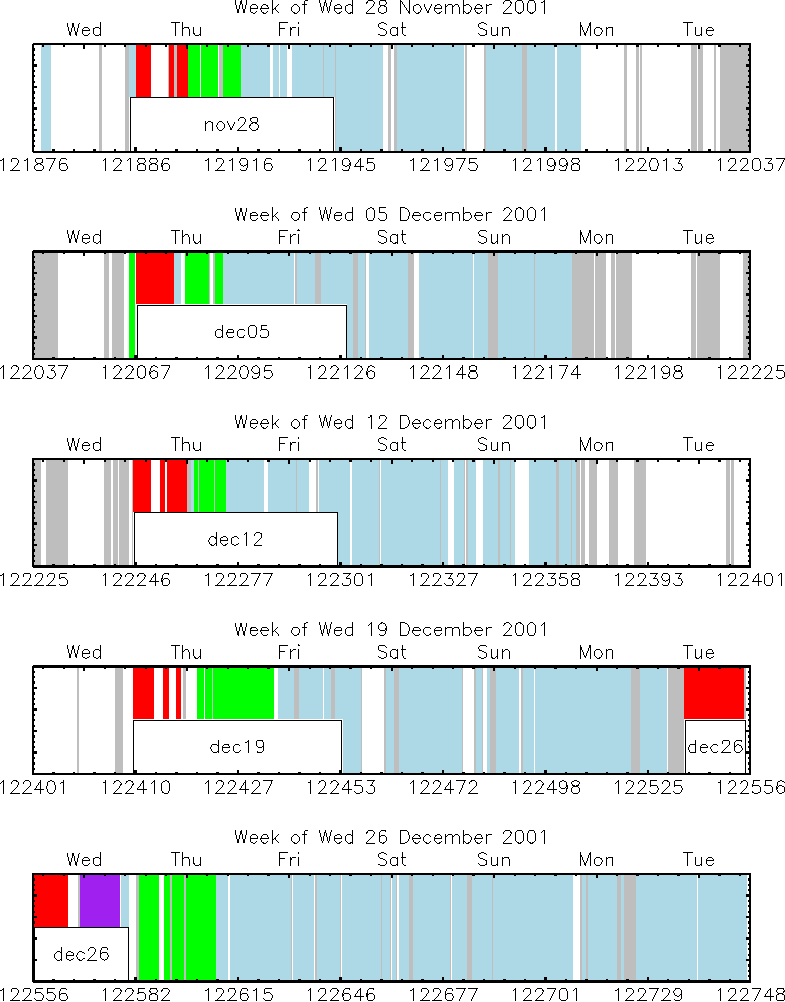
\includegraphics[width=0.95\linewidth]{scan_periods1}
  \caption{\label{scanperiods1} Run periods by date and run number
  (1).  Red regions are off-resonance scan, blue are on the top of the
  resonance peak ($\pm$ 0.8 MeV), green are off-resonance continuum
  ($\sim$10 MeV below resonance), purple are high-energy tail
  measurements (25--50 MeV above resonance), grey are not DataTaking
  runs in the $\Upsilon$ region, and white spaces are between runs or
  are runs without StartRun/EndRun timestamps.}
\end{figure}

\begin{figure}[p]
  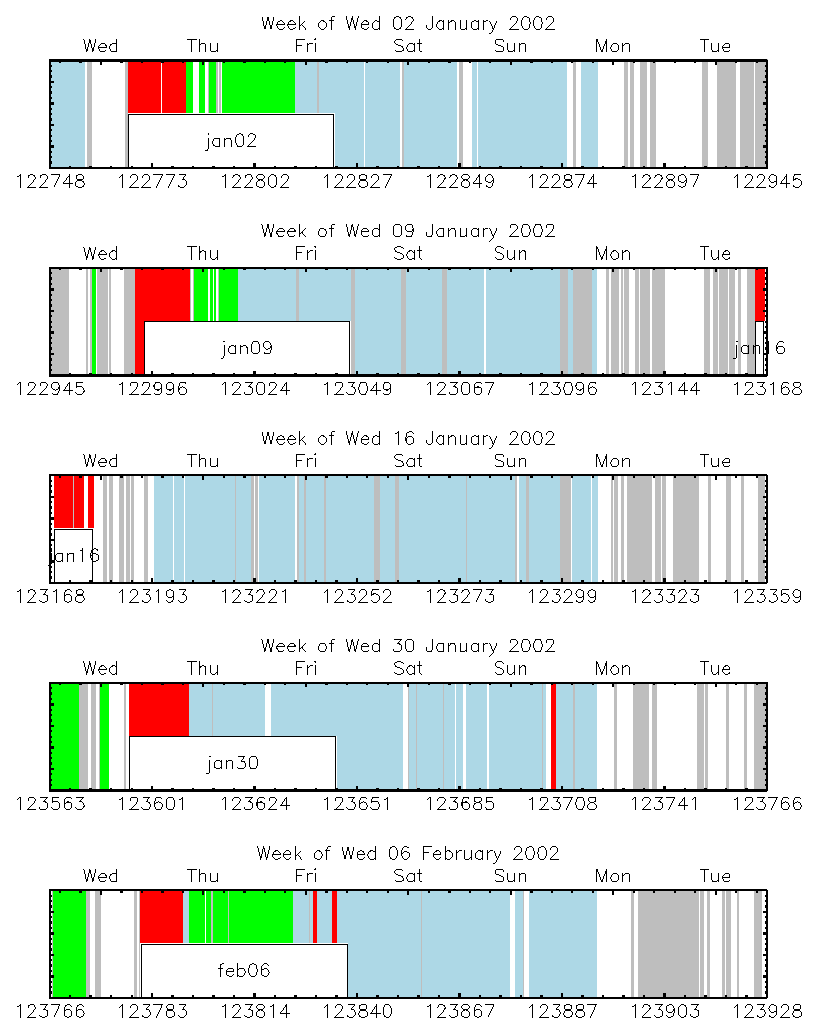
\includegraphics[width=0.95\linewidth]{scan_periods2}
  \caption{\label{scanperiods2} Run periods by date and run number
  (2).  See Figure \ref{scanperiods1} caption for color
  designations.  The red region just before jan09 was an \uone\ test.}
\end{figure}

\begin{figure}[p]
  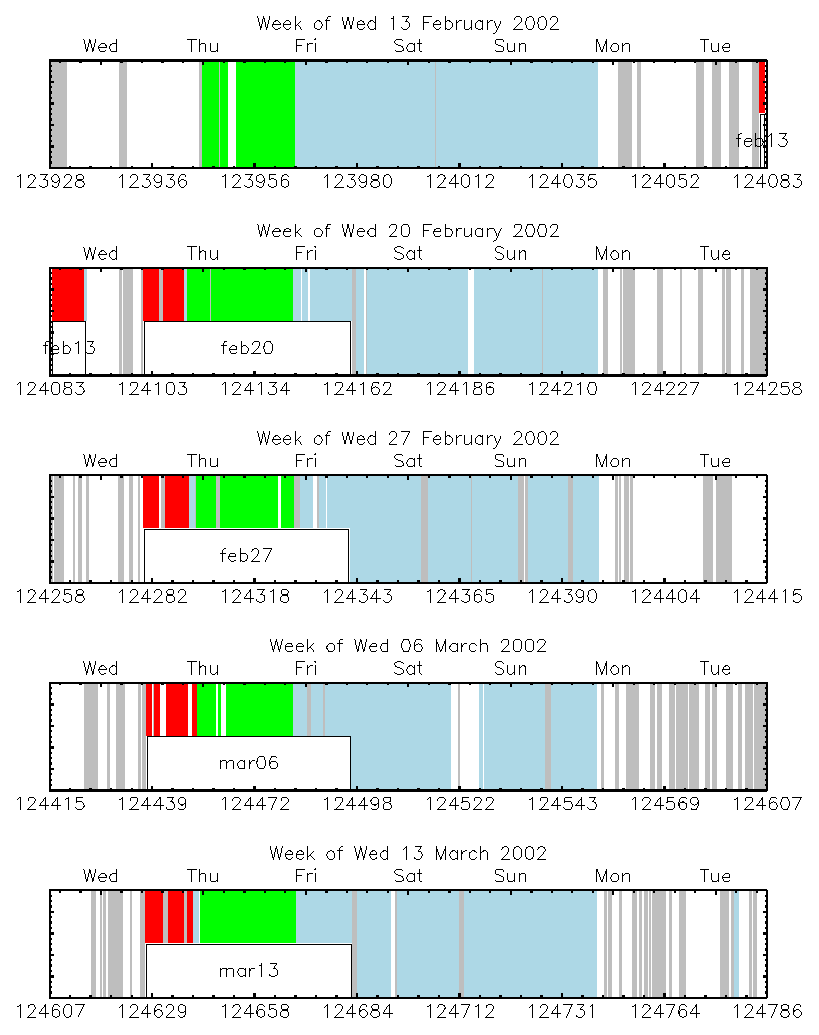
\includegraphics[width=0.95\linewidth]{scan_periods3}
  \caption{\label{scanperiods3} Run periods by date and run number
  (3).  See Figure \ref{scanperiods1} caption for color
  designations.}
\end{figure}

\begin{figure}[p]
  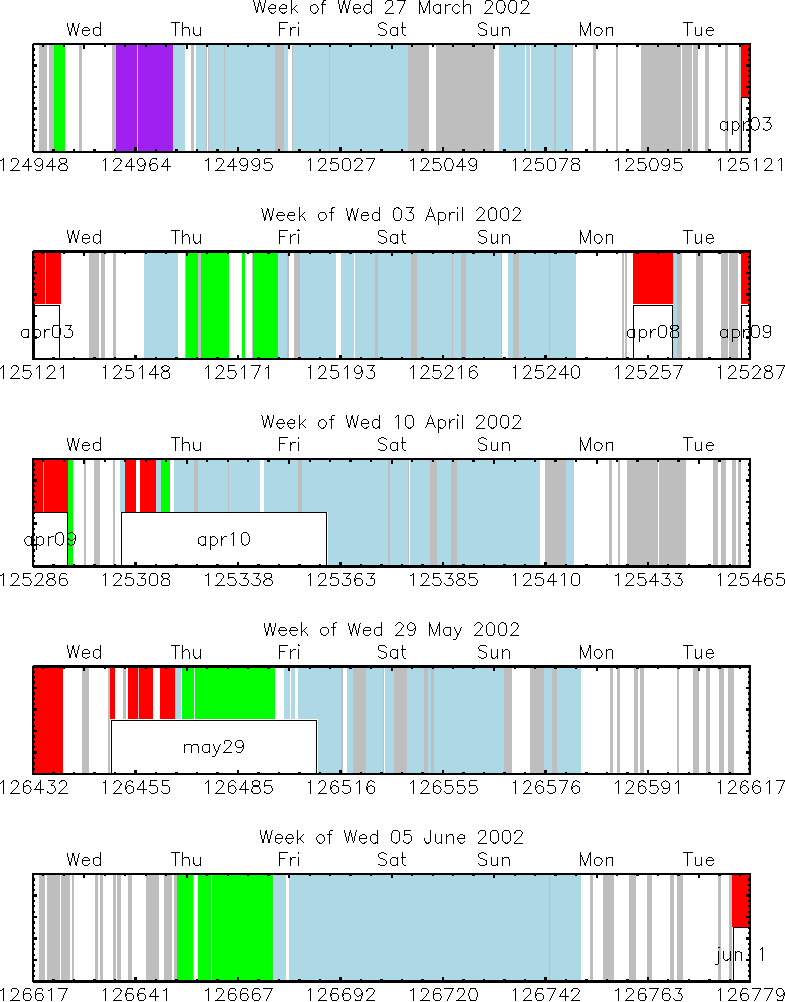
\includegraphics[width=0.95\linewidth]{scan_periods4}
  \caption{\label{scanperiods4} Run periods by date and run number
  (4).  See Figure \ref{scanperiods1} caption for color
  designations.  The red region before may29 was a \utwo\ test.}
\end{figure}

\begin{figure}[p]
  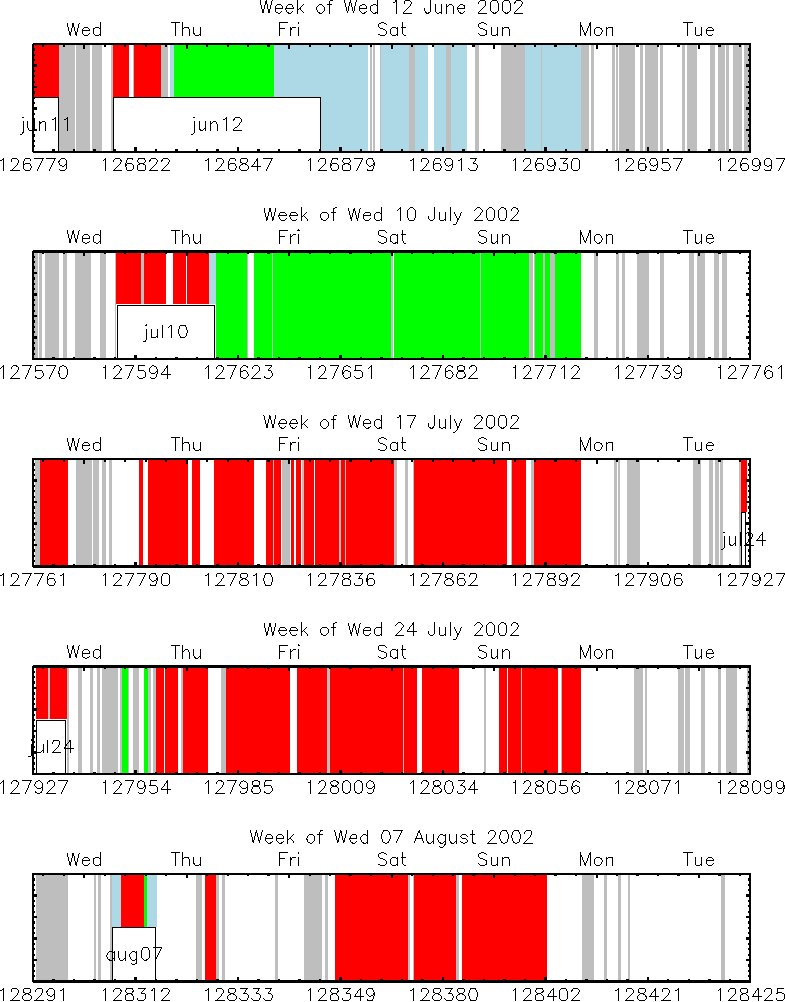
\includegraphics[width=0.95\linewidth]{scan_periods5}
  \caption{\label{scanperiods5} Run periods by date and run number
  (5).  See Figure \ref{scanperiods1} caption for color
  designations.  The unassigned red regions on this plot are near the
  top of the \uthree\ peak, and don't constitute a full scan.}
\end{figure}

%% is this an even page or an odd page?
%% if even, you want angle=-90
\begin{figure}[p]
  \includegraphics[height=0.9\linewidth, angle=-90]{../plots/all25}
  \caption{\label{postage} Plots of individual scans, showing what
    energy points were available to each.  The unlabeled axes do not
    share the same scale: for measured mass and beam energy spread
    values, see Figures \ref{centroids} and Figure \ref{widths} and
    the text.}
\end{figure}

\end{document}
